\subsection*{Présentation de la base \emph{mroz}.}

La base \emph{mroz} est une base composée 753 individus et de 22 variables. Elle présente un échantillon de femmes mariées et leurs activités sur le marché du travail aux États-Unis. Cette base permet de couvrir des thématiques variées telle que la participation ou non au marché du travail, leurs caractéristiques personnelles telles que l'âge, leur situation familiale (nombre d'enfants) ou bien des caractéristiques relatives à leur conjoint... 

\vspace*{0.3cm}

Pour l'analyse qui va suivre (partie 1), nous allons nous concentrer sur dix variables : \emph{inlf} qui étudie la participation ou non de la femme $i$ au marché du travail. \emph{Nwifeinc} qui présente le revenu du ménage hors salaire de la femme, cette variable comprends le revenu du patrimoine ainsi que le revenu du conjoint. En d'autres termes, c'est le revenu de transfert. Les variables éducation (\emph{educ}) et expérience (\emph{exper}) qui retracent le parcours de l'individu. Nous sélectionnons aussi l'âge (\emph{age}) de l'individu. Et enfin, nous disposons de deux variables rapportant le nombre d'enfants de l'individu (la première variable (\emph{kidslt6}) traite des enfants ayant un âge inférieur à 6 ans et la seconde traite du nombre d'enfants ayant un âge compris entre 6 et 18 ans.)

\vspace*{0.3cm}

Dans la question 8 (modèle de sélection et modèle de comptage), nous ajoutons les variables \emph{hours} et \emph{hushrs} qui quantifient respectivement le nombre d'heures travaillés par la femme et celles travaillées par son conjoint.


%%%%%%%%%%%%%%%%%%%%%%%%%%%%%%%%%%%%%



\subsection{Statistiques descriptives de la base \emph{mroz}.}

\begin{figure}[h]
    \caption{Statistiques descriptives en fonction de la participation au marché du travail.}
    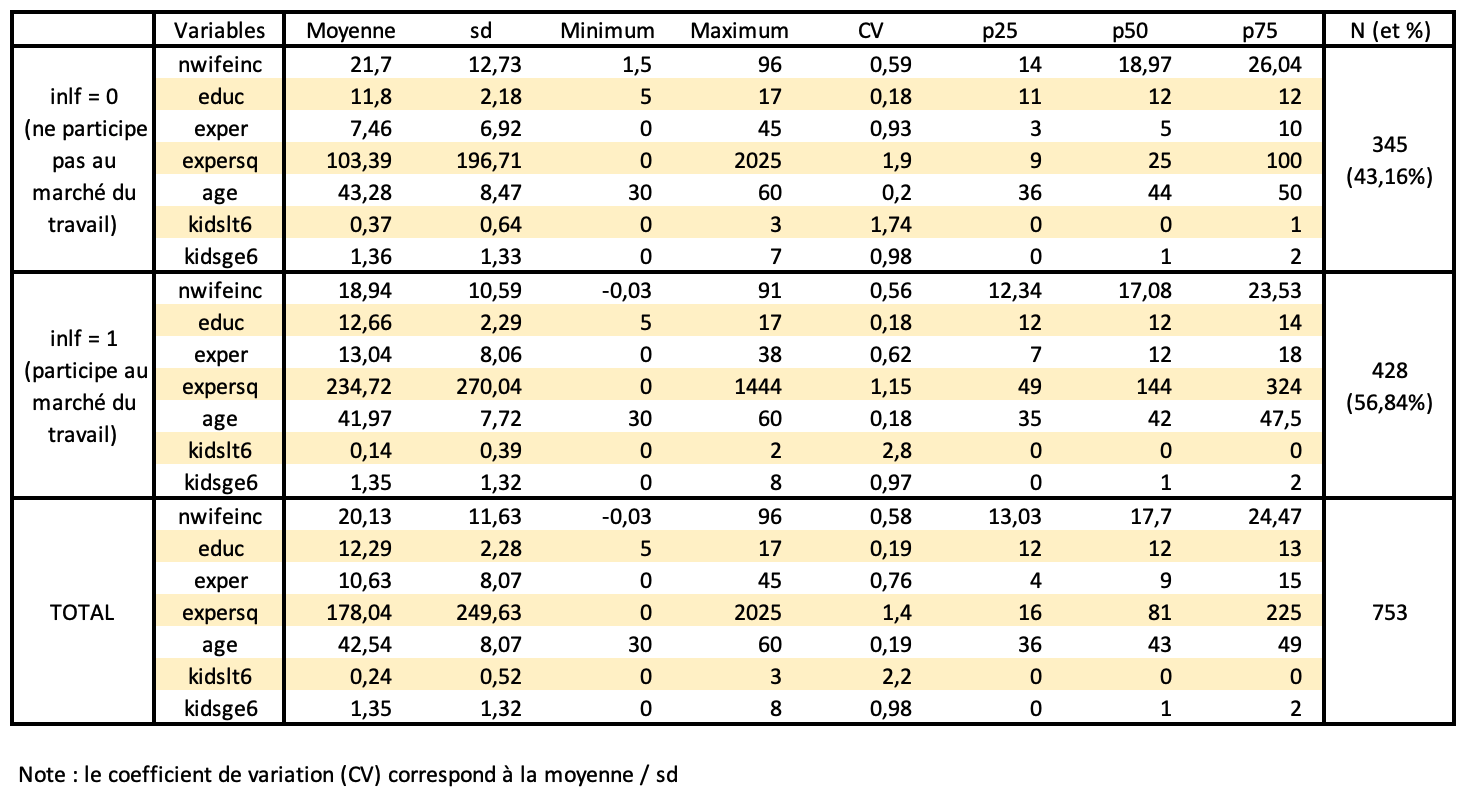
\includegraphics[scale = 0.65]{101_graphics/11_Stats_desc.png}
    \centering
    \label{fig:StatsDesc}
\end{figure}

%%%%%%%%%%%%%%%%%%%%%%%%%%%%%%%%%%%%%




\subsection{Les effets attendus des variables.}

\subsubsection*{Revenu de transfert ou \emph{nwifeinc}.}

La variable \emph{Nwifeinc} décrit le revenu du ménage une fois enlevé le revenu de la femme. Il comprend alors les revenus du patrimoine et les revenus du travail du conjoint. Nous attendons un effet négatif de cette variable : plus le revenu du ménage augmente, moins la probabilité de travailler de la femme est important. Nous pouvons imaginer que si le revenu du ménage est faible alors, la femme doit contribuer par son travail à la richesse du ménage pour répondre aux besoins du ménage. Le coût d’opportunité de travail est de moins en moins important avec l’augmentation du revenu du ménage hors salaire de la femme. Nous pouvons illustrer avec les statistiques descriptives : le revenu du ménage hors salaire de la femme chez les individus qui travaillent est inférieur au revenu moyen des ménages des individus qui travaillent (21,7 contre 18,9). Nous pouvons vérifier que ces des moyennes sont significativement différentes en appliquant un test d’égalité des moyennes. La probabilité critique associée à ce test ($p_value = 0.0012$) est inférieur à 5\%, nous rejetons alors hypothèse nulle d’égalité des moyennes, nous pouvons alors déduire que les deux moyennes sont significativement différentes.

\subsubsection*{Education (\emph{educ}).}

Nous attendons un effet positif de l’éducation sur la probabilité de travailler pour deux raisons principalement. Les femmes éduquées sont exposées à des périodes de chômage plus courte. Le taux de chômage parmi les non-diplômés est supérieur à celui des individus éduqués. Une deuxième explication qui va dans le même sens : après avoir supporté les coûts de l’éducation c'est-à-dire le coût financier des études ainsi que le coût d’opportunité (le coût de ne pas travailler), l’individu cherche à valoriser les enseignements de son parcours éducations en cherchant un emploi. Nous pouvons alors penser qu’il existe chez l’individu qui travaille, une volonté grande de trouver un emploi à la suite de ces études. 

\subsubsection*{Expérience (\emph{exper}).}


Nous anticipons un effet positif de l’expérience sur la probabilité de travailler. Un individu ayant de l’expérience a acquis par la pratique des compétences qu’il peut valoriser sur le marché du travail le rendant alors moins sensible aux phases de chômage (pour les employeurs, son expérience est un actif intéressant). De plus, nous pouvons imaginer qu’une personne ayant de l’expérience dans son activité, a une connaissance fine du marché (relation tissée par exemple) et compétences propres au secteur.

\subsubsection*{Expérience au carré ou \emph{expersq}.}

Nous attendons un effet négatif sur l’expérience mis au carré. La variable expersq permet de mettre en évidence une relation non linéaire entre l’expérience et la probabilité de travailler. Le signe attendu est négatif puisque que nous imaginons une fonction est concave (admet un maximum). En d’autres termes, une année d’expérience supplémentaire permet d’augmenter la probabilité de travailler, de plus en plus jusqu’à un certain point. A ce point, une année supplémentaire d’expérience se traduit par une augmentation de la probabilité de travailler moins grande qu’à la période précédente. Nous pouvons interpréter cela par l’obsolescence des compétences. Une personne ayant un grand nombre d’année dans le secteur peut manquer de perspective et d’un certain recul. En d’autres termes, la productivité de l’individu décroche, le rendant un peu moins attractif. 

\subsubsection*{Âge.}

L’effet de l’âge est indéterminé. Nous pouvons imaginer deux relations évoluant en sens inverse. La première relation est positive. Nous pouvons imaginer une discrimination à l’embauche de la part des employeurs envers des jeunes femmes (entre 20 et 30 ans), anticipant une potentielle maternité dans les années à venir ou bien une autre situation : l’employeur s’appuie le stéréotype suivant : les femmes sont première donneuse de soin à leur enfant en cas de maladie, préfèrera un homme (réduisant alors l’employabilité de la femme) (Petit 2003). L’âge avançant, cette contrainte potentielle se lève. Un accroissement de l’âge aura un effet positif sur la probabilité de travailler. Nous pouvoir imaginer aussi un effet négatif, une discrimination négative contre les séniors. Les employeurs anticipant le départ à la retraite des individus âgés préfèrent sélectionner des individus plus jeunes. La question est de savoir quel effet l’emporte sur l’autre.

\begin{figure}[h]
    \caption{Évolution de la probabilité de travailler pour une femme en fonction du nombre d'années d'expérience dans le poste actuel.}
    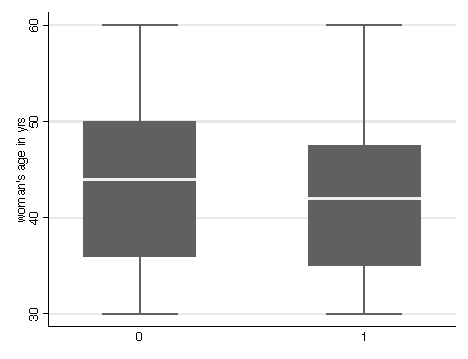
\includegraphics{101_graphics/boxplot.pdf}
    \centering
    % \label{fig:EvolutionDelaProbabilitéEnFonctionDesAnnées}
\end{figure}

Les deux boîtes à moustaches montrent que les femmes qui travaillent sont plus jeunes (en s'appuyant sur le premier quartile, la médiane et le troisième quartile).

\subsubsection*{Nombre d'enfants sous 6 ans ou \emph{kidslt6}.}

La variable \emph{Kidslt6} indique le nombre d’enfants âgés de moins de 6 ans. Nous imaginons un effet négatif de cette variable sur la probabilité de travailler. Deux raisons : la première est sociologique, souhaitant s’occuper de ses jeunes enfants (pour des raisons économiques ou personnelles), la femme peut choisir d’arrêter de travailler. Une seconde raison est économique : des inégalités salariales existe entre homme et femme, une femme renonçant à travailler, elle renonce à un salaire moins élevé que si l’homme s’arrêtait. Le choix devient économiquement pertinent pour le ménage. 

\subsubsection*{Nombre d'enfants entre 6 ans et 18 ans ou \emph{kidsge6}.}

La variable \emph{Kidsge6} décrit le nombre d’enfant ayant plus de 6 ans tout en ayant moins de 18 ans. Nous attendons un effet interdéterminé sur la probabilité de travailler de la femme. En effet, nous anticipons un effet positif du nombre d’enfants sur la probabilité de travailler : avec le nombre d’enfants augmentant, les charges associées augmentent. De plus, cette tranche d’âge correspond à l’âge de l’école, la mère peut alors travailler. Néanmoins, nous pouvons aussi imaginer un effet négatif, la mère peut toujours envie de s’occuper de ses enfants (raisons personnelle et économique). Nous pouvons faire la remarque que cette catégorie est hétérogène : les besoins ne sont les mêmes entre un enfant de 6 ans et un enfant de 18 ans. Cela interroge sur l’interprétation donné au test Nous pouvons montrer cela en réalisant un simple test du $\chi^2$ (indépendance entre les deux variables). Nous trouvons une $p_value$ supérieur à 5\% ($Pr = 0.763$), nous ne pouvons donc pas rejeter l’hypothèse nulle d’indépendance.

%%%%%%%%%%%%%%%%%%%%%%%%%%%%%%%%%%%%%



\subsection{Estimation des modèles Logit, Probit et le modèle de probabilité linéaire.}

\subsection*{Le modèle \emph{Logit}.}

\subsubsection*{Présentation théorique du modèle.}

Nous allons estimer le modèle suivant : 

\begin{align*}
   p_i = & \frac{e^{\beta_0 + \beta_1 \cdot nwifeinc_i + \beta_2 \cdot educ_i + \beta_3 \cdot exper_i + \beta_4 \cdot exper_i^2 + \beta_5 \cdot age_i + \beta_6 \cdot kidslt6_i + \beta_7 \cdot kidsab6_i}}{1+e^{\beta_0 + \beta_1 \cdot nwifeinc_i + \beta_2 \cdot educ_i + \beta_3 \cdot exper_i + \beta_4 \cdot exper_i^2 + \beta_5 \cdot age_i + \beta_6 \cdot kidslt6_i + \beta_7 \cdot kidsab6_i}}
\end{align*}

Ici, nous pouvons voir qu'une probabilité sera associée à chaque individu. Le modèle est par nature hétéroscédastique, pour les analyses puisque la variance est dépendante de l'individu $i$. 

\subsubsection*{Estimation du modèle Logit.}

\begin{figure}[h]
    \caption{Regression du modèle Logit dichotomique participation des femmes au marché du travail.}
    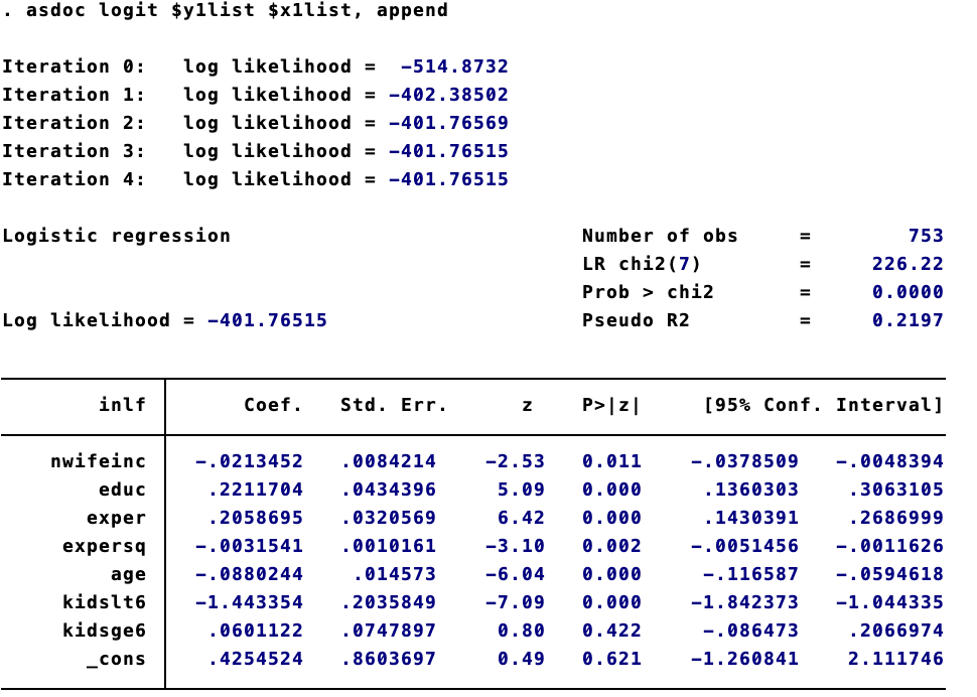
\includegraphics[scale = 0.8]{100_tab_results/partie1logitdicho.png}
    \centering
    \label{reg:Logitdichotomique}
\end{figure}


Le modèle \ref{reg:Logitdichotomique} est estimé avec la méthode du maximum de vraisemblance. Le modèle est globalement significatif au seuil de 5\% et son pouvoir explicatif est satisfaisant (un pseudoR2 a presque 22\%). Tous les coefficients sont significatifs à l’exception de la variable kidsge6 qui présente le nombre d’enfants âgés entre 6 et 18 ans. Nous pouvons interpréter les signes des coefficients tout d’abord : le revenu de transfert a un effet négatif sur la probabilité de travail, l’éducation et l’expérience ont un effet positif. Le coefficient associé l’expérience au carré est négatif mettant en évidence la relation non constante de l’expérience (une relation en forme de cloche qui admet un maximum). Concernant l’âge, l’effet négatif l’emporte sur le positif. Enfin avoir un enfant ayant moins de 6 ans réduit la probabilité de travailler pour la femme. Nous retrouvons les effets identifiés a priori. Les coefficients peuvent être interprétés comme des semi-élasticité mais l’interprétation avec les odd ratio (transformation exponentielle des coefficients) est plus accessible. 


\subsection*{Le modèle \emph{Probit}.}

\subsubsection*{Présentation théorique du modèle.}

Nous allons estimer le modèle suivant : 

\begin{align*}
    p_i = \frac{1}{\sqrt{2\pi}} \cdot e^{\frac{(\beta_0 + \beta_1 \cdot nwifeinc_i + \beta_2 \cdot educ_i + \beta_3 \cdot exper_i + \beta_4 \cdot exper_i^2 + \beta_5 \cdot age_i + \beta_6 \cdot kidslt6_i + \beta_7 \cdot kidsab6_i)^2}{2}}
 \end{align*}

 \subsubsection*{Estimation du modèle Probit.}

 \begin{figure}[h]
    \caption{Regression du Probit dichotomique : participation des femmes au marché du travail.}
    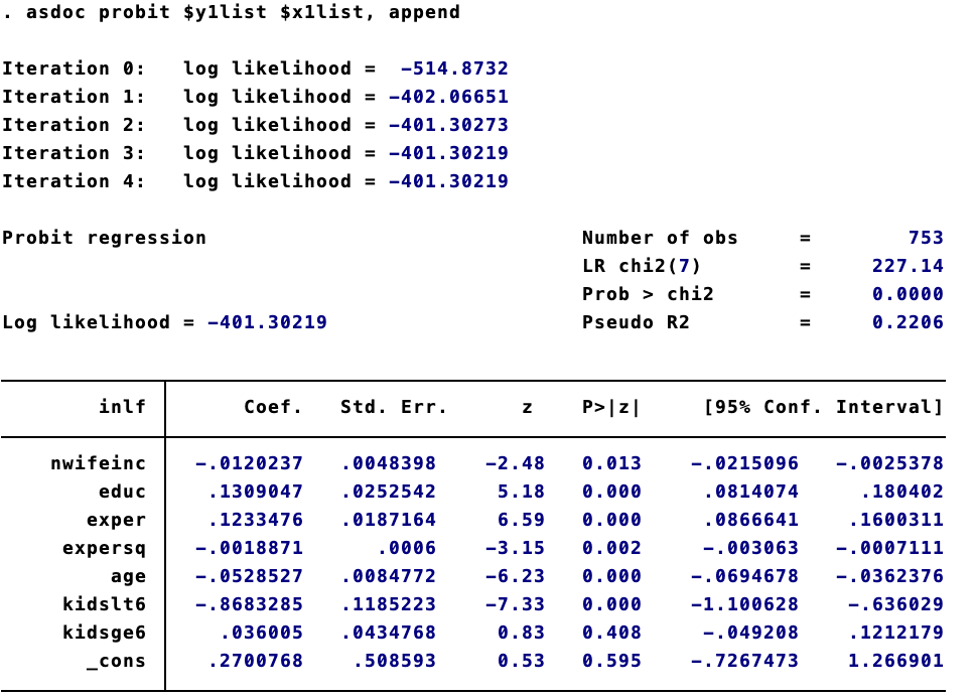
\includegraphics[scale = 0.8]{100_tab_results/probitdicho.png}
    \centering
    \label{reg:Probitdichotomique}
\end{figure}

 Le probit \ref{reg:Probitdichotomique} s’estime lui aussi à l’aide de la méthode du maximum de vraisemblance. Le modèle est globalement significatif. Le pseudo R2 est égal à 22\%, ce qui est satisfaisant. Tous les coefficients sont significatifs à l’exception de la variable kidsge6. Les coefficients ne sont pas directement interprétables, nous devons utiliser les effets marginaux. Néanmoins, nous pouvons interpréter les signes des coefficients. Nous retrouvons les résultats du logit présenté un peu plus haut.

 \subsection*{Le modèle de \emph{probabilité linéaire}.}

 \subsubsection*{Présentation théorique du modèle.}

 Nous allons estimer l'équation suivante : 
 
 \begin{align*}
     Y = & X \beta + \varepsilon  &  \varepsilon \backsim N(0,\sigma^2_{\varepsilon})  \nonumber \\
     y_i  = & \beta_0 + \beta_1 \cdot nwifeinc_i + \beta_2 \cdot  educ_i + \beta_3 \cdot exper_i + \beta_4 \cdot exper_i^2 + \nonumber \\ 
     & \beta_5 \cdot age_i + \beta_6 \cdot kidslt6_i + \beta_7 \cdot kidsab6_i + \varepsilon_i 
 \end{align*}

 \subsubsection*{Estimation du modèle de probabilité linéaire.}

 Le modèle de probabilité linéaire est une adaptation du modèle MCO au cadre probabiliste. Il s’agit d’une estimation par les moindres carrés (nous cherchons à minimiser la somme des carrés des résidus). 

\begin{figure}[h]
    \caption{Regression MCO (modèle de probabilité linéaire) : participation des femmes au marché du travail.}
    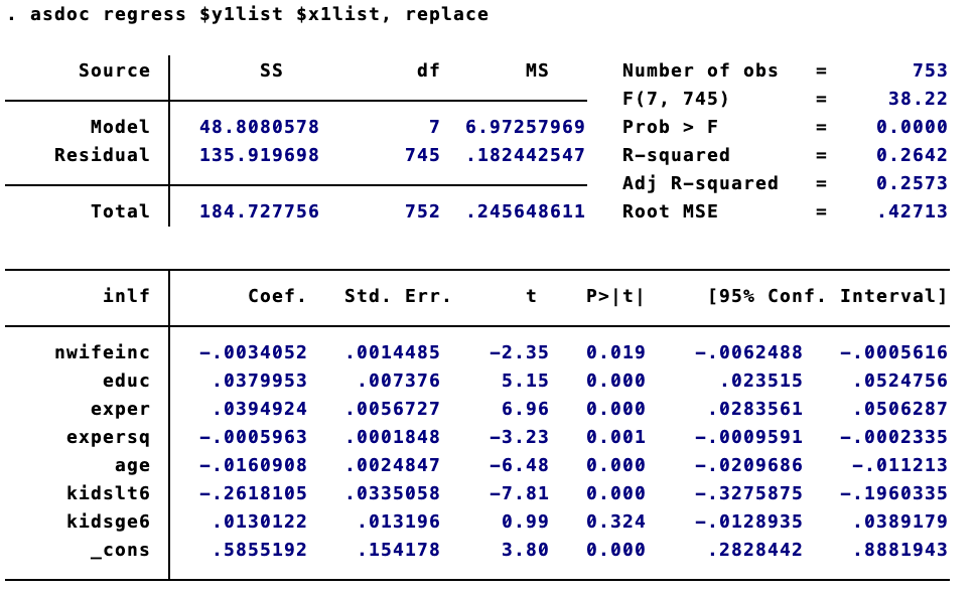
\includegraphics[scale = 0.8]{100_tab_results/probalineaire.png}
    \centering
    \label{reg:linearProba}
\end{figure}


 Le modèle \ref{reg:linearProba} est globalement significatif mais a une capacité d’explication limitée (le R2 ajusté n’est que de 25,73\% bien inférieur au seuil de 50\%). Toutes les variables sont significatives à l’exception de la variable kidsge6. Les coefficients sont directement interprétables comme des effets marginaux. Ainsi, lorsque le revenu de transfert augmente de 1, la probabilité de travailler pour la femme diminue de 0,0034 point de pourcentage. Une année d’éducation supplémentaire provoque une augmentation de la probabilité de travailler pour la femme de 0,03 point de pourcentage. L’expérience a un effet positif sur la probabilité de travailler (+0,039 points de pourcentage), mais la relation n’est pas constante et admet un maximum (le coefficient associé à la variable expersq). L’âge a un effet négatif sur la probabilité de travailler et avoir un enfant de moins de 6 ans joue négativement (-0.26 points de pourcentage).
Nous obtenons des résultats cohérent entre les trois modèles (même signes).Néanmoins, le dernier modèle estimé présente des limites.


%%%%%%%%%%%%%%%%%%%%%%%%%%%%%%%%%%%%%


\subsection{L'emploi du modèle de probabilité linéaire.}

Le modèle linéaire peut être utilisé dans un premier temps pour identifier des effets au préalable des différents régresseurs sur la variable d’intérêt et permettre de sélectionner les variables notamment en s’appuyant sur la significativité de ces dernières. Le modèle MCO présente directement les effets marginaux contrairement au logit et au probit. 

\vspace*{0.3cm}

Néanmoins au-delà de facilité de l'utilisation, ce modèle présente des limites. La première limite est graphique. La variable d’intérêt ne peut prendre que deux valeurs. La droite de régression (dans la mesure d’une représentation possible avec plus de 2 variables explicatives) ne va pas pouvoir ajuster le nuage de points de manière satisfaisante. De plus, les valeurs prises par la variable endogène n’ont pas de sens en soit, elles n’indique que des modalités. Or, l’estimateur des MCO se construit sur les valeurs de la variable endogène : $\beta = (X'X)^{-1}X'y$. 

\vspace*{0.3cm}

La seconde limite porte sur les résidus. La valeur $\varepsilon_i$ peut prendre deux valeurs : 

 \begin{equation*}
	\left\lbrace
		\begin{aligned}
            Si \: \: y_i = 1  \:\:\:\:\:\:\: alors \:\:\:\:\:\:\: & \varepsilon_i = 1 - x_i\beta \\
            Si \: \:y_i = 0  \:\:\:\:\:\:\: alors \:\:\:\:\:\:\: & \varepsilon_i = -x_i\beta \\
		\end{aligned}
	\right.
\end{equation*}


 Nous calculons désormais l'espérance conditionnelle de l'erreur en rappelant l'hypothèse sur le terme d'erreur que pose le modèle des MCO $E(\varepsilon_i,X_i = x_i) =0$.

\begin{align*}
   E(\varepsilon_i | X_i = x_i) &= \: \: p_i (1 - x_i\beta) + 1- p_i (- x_i\beta) \\
   E(\varepsilon_i | X_i = x_i) &= \: \: p_i - x_i\beta \\ 
   &E(\varepsilon_i | X_i = x_i) = 0 \\
    &p_i - x_i\beta = 0 \\ 
    &p_i = x_i\beta 
\end{align*}

Une probabilité doit être compris entre 0 et 1, rien n'assure que $x_i\beta$ ne soit compris entre 0 et 1. Nous pouvons vérifier ce principe dans notre cas avec la représentation suivante : 

\begin{figure}[h]
    \caption{Répartition des probabilités selon le modèle de probabilité linéaire.}
    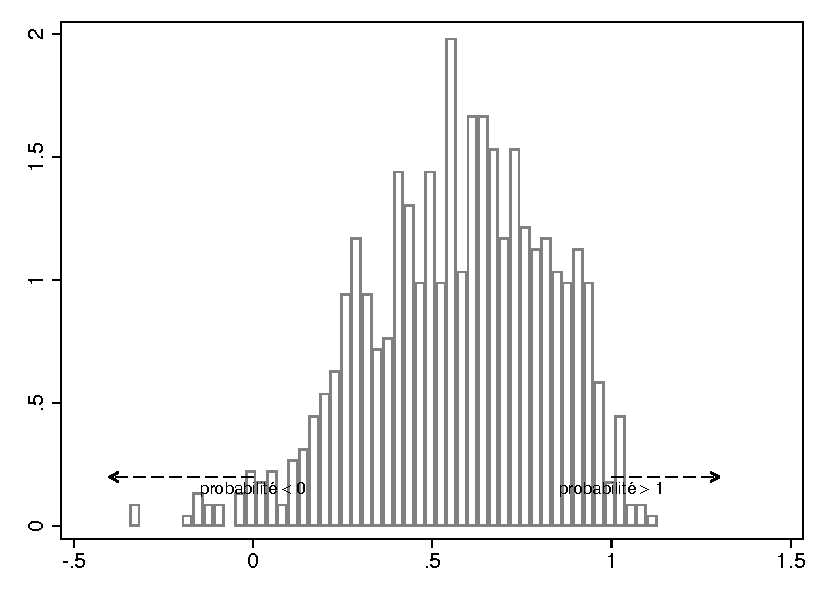
\includegraphics[scale = 0.7]{101_graphics/histogram_yhat.pdf}
    \centering
    \label{fig:ProbaEntre0et1}
\end{figure}


Nous pouvons voir sur cette figure \ref{fig:ProbaEntre0et1}, qu'il existe des valeurs de probabilité qui n'appartiennent pas à l'intervalle $[0,1]$. Pour faire face à ce problème, nous pourrions modifier les valeurs des probabilités pour qu'elles prennent les valeurs extrêmes (0 et 1). Cette solution n'est pas entièrement satisfaisante, les modèles Logit et Probit semblent être plus intéressant.  

\vspace*{0.3cm}

Enfin, l’estimateur des MCO est ici hétéroscédastique. C'est-à-dire que la variance dépend des individus. Cette contrainte peut être levée en considérant des estimateurs robustes (EQMV avec une forme \emph{Sandwitch}).


%%%%%%%%%%%%%%%%%%%%%%%%%%%%%%%%%%%%%


\subsection{Les effets marginaux des variables sur la probabilité de travailler.}

Dans cette section il s'agit d'étudier les effets marginaux décrits dans les modèles Logit et Probit.


\begin{center}
    \small
    \begin{table}[htbp]\centering
\def\sym#1{\ifmmode^{#1}\else\(^{#1}\)\fi}
\caption{Effets marginaux des modèles logit et probit}
\begin{tabular}{l*{2}{c}}
\hline\hline
                    &\multicolumn{1}{c}{(1)}&\multicolumn{1}{c}{(2)}\\
                    &\multicolumn{1}{c}{mfx Logit}&\multicolumn{1}{c}{mfx Probit}\\
\hline
=1 if in lab frce, 1975&                     &                     \\
HouseInc-womanWage  &     -0.0213\sym{*}  &     -0.0120\sym{*}  \\
                    &     [-2.53]         &     [-2.48]         \\
[1em]
years of schooling  &       0.221\sym{***}&       0.131\sym{***}\\
                    &      [5.09]         &      [5.18]         \\
[1em]
Actual experience   &       0.206\sym{***}&       0.123\sym{***}\\
                    &      [6.42]         &      [6.59]         \\
[1em]
ExperienceSq        &    -0.00315\sym{**} &    -0.00189\sym{**} \\
                    &     [-3.10]         &     [-3.15]         \\
[1em]
woman's age in yrs  &     -0.0880\sym{***}&     -0.0529\sym{***}\\
                    &     [-6.04]         &     [-6.23]         \\
[1em]
kids < 6y           &      -1.443\sym{***}&      -0.868\sym{***}\\
                    &     [-7.09]         &     [-7.33]         \\
[1em]
kids 6 - 18y        &      0.0601         &      0.0360         \\
                    &      [0.80]         &      [0.83]         \\
[1em]
Constant            &       0.425         &       0.270         \\
                    &      [0.49]         &      [0.53]         \\
\hline
Observations        &         753         &         753         \\
\hline\hline
\multicolumn{3}{l}{\footnotesize \textit{t} statistics in brackets}\\
\multicolumn{3}{l}{\footnotesize \sym{*} \(p<0.05\), \sym{**} \(p<0.01\), \sym{***} \(p<0.001\)}\\
\end{tabular}
\end{table}

    \normalsize
\end{center}


%%%%%%%%%%%%%%%%%%%%%%%%%%%%%%%%%%%%%


\subsection{Probabilité de travailler et expérience.}

Graphiquement, nous représentons l'évolution de la probabilité de travailler pour une femme aux États-Unis (en 1975) lorsque nous faisons évoluer le nombre d'année d'expérience dans le poste actuel. 

\begin{figure}[!h]
    \caption{Évolution de la probabilité, de la côte et du odd-ratio de travailler pour une femme en fonction du nombre d'années d'expérience dans le poste actuel.}
    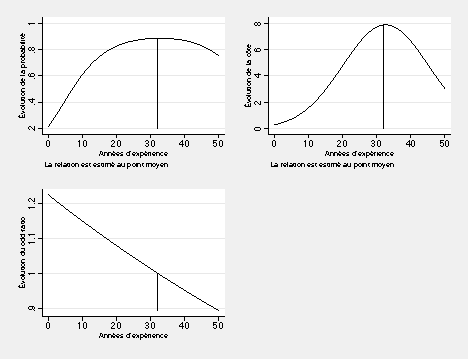
\includegraphics[scale = 1.5]{101_graphics/EvoProbaExperience.pdf}
    \centering
    \label{fig:EvolutionDelaProbabilitéEnFonctionDesAnnées}
\end{figure}

De manière évidente dans la figure \ref{fig:EvolutionDelaProbabilitéEnFonctionDesAnnées}, la relation n'est pas linéaire, elle a la forme d'une cloche (une fonction concave). Cela signifie que jusqu'à un certain seuil, une année d'expérience supplémentaire dans le poste actuel accroit la probabilité de participer au marché du travail, après, une année supplémentaire fait diminuer la probabilité supplémentaire de travailler. 

\vspace*{0.3cm}

Pour le calcul du seuil, c'est-à-dire le niveau où une année d'expérience supplémentaire n'accroit plus la probabilité de travailler, nous cherchons le niveau d'expérience qui donne un \emph{odd-ratio} égal à 1, alors nous posons les opérations suivantes : 
 
\begin{align}
    OR_{experience} & =  \frac{\frac{p_1}{1-p_1}}{\frac{p_0}{1-p_0}}  =  \frac{p_1}{1-p_1} \cdot \frac{1-p_0}{p_0}  = 1 & \nonumber \\
    % ou OR_{experience} & =  \frac{p_1}{1-p_1} \cdot \frac{1-p_0}{p_0}     = 1 & \nonumber\\
    & =  e^{\beta_1 + 2 \cdot \beta_2 \cdot exper_{seuil} + \beta_2} =1 & \nonumber \\
    log(OR_{experience}) & =  \beta_1 + 2 \cdot \beta_2 \cdot exper_{seuil} + \beta_2 = 0  &\nonumber \\ 
    exper_{seuil} & =  - \frac{\beta_1 + \beta_2}{2 \cdot \beta_2} \nonumber
\end{align}

En remplaçant les coefficients par leur valeur trouvée dans la régression Logit, nous pouvons en déduire les résultats suivants : 


\begin{align}
    &exper_{seuil} =  32.13 \nonumber \\
    &p_{seuil} = 12.34 \nonumber 
\end{align}


%%%%%%%%%%%%%%%%%%%%%%%%%%%%%%%%%%%%%



\subsection{\emph{kidslt6}, une variable endogène ?}

Il existe quatre raisons de l’endogénéité : hétérogénéité inobservée, causalité inverse, causalité commune, erreur de mesure sur les variables explicatives. Économétriquement, l’endogénéité se traduit par la relation suivante : 

\begin{align*}
    cov(X_i \: | \: \varepsilon_i) \ne 0  
\end{align*}

L’endogénéité va biaiser les résultats. Dans notre cas, nous suspectons de l’endogénéité portée par la variable kidslt6 pour plusieurs raisons. Tout d’abord, nous pouvons indiquer qu’il existe une relation entre la variable kidslt6 et les autres variables du modèle dont notamment âge, l’expérience, l’éducation, le nombre d’enfant âgé de plus de 6 ans. Nous pouvons illustrer avec une simple régression MCO. La régression est globalement significative et l’ensemble des variables sont significativement différents de 0 au seuil de 5\%. 
%%%%%%%%%%%%%%%%%%%%%%%%%%%%%%%%%%%%%



\subsection{Expliquer le nombre d'heures travaillées (\emph{hours}).}



\subsubsection{Le rôle de la variable \emph{hurshrs}.}

Le nombre d’heures travaillés par le conjoint peut être utilisé pour mesurer l’engagement familial du conjoint. De cette manière, le conjoint présentant un nombre d’heure faible, peut signifier davantage disponibilité pour la femme lui permettant de travailler. Nous attendons alors un effet négatif, les deux variables évoluant en sens inverse. Une autre explication, un conjoint travaillant peu, peut signifier que la femme doit trouver un travail pour répondre aux besoins du foyer. 

\vspace*{0.3cm}

L’interaction entre l’éducation et l’expérience va permettre de capter un effet joint de ces deux variables et de mettre en évidence la conjugaison des deux effets (forte expérience et forte éducation). Aussi, nous pouvons imaginer deux situations que cette variable va capter : des jeunes arrivant sur le marché du travail (peu d’expérience et un niveau d’éducation élevé), tout comme des personnes ayant de l’expérience sans avoir un niveau d’éducation élevé.

\subsubsection{Modèle MCO sur les travailleurs.}

\begin{figure}[h]
    \caption{Regression MCO sur les travailleurs.}
    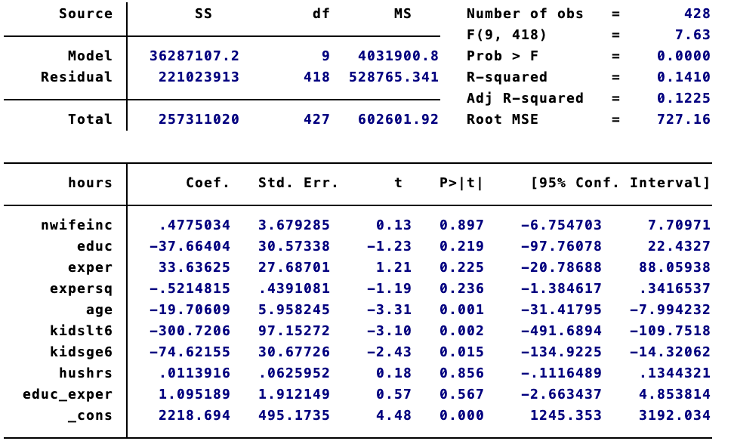
\includegraphics[scale = 0.8]{100_tab_results/MCOsurlestravailleurs.png}
    \centering
    \label{reg:MCOtravailleurs}
\end{figure}


En estimant seulement les individus qui travaillent \ref{reg:MCOtravailleurs}, nous avons une sous-population spécifique avec des caractéristiques qui lui sont propres qui sont inobservables dans notre modèle considéré. Les estimateurs sont biaisés (biais de sélection), nous ne pouvons pas en déduire des résultats globaux pour la population. En d’autres termes, nous ne pouvons utiliser le principe de l’inférence. 

\subsubsection{Modèle MCO sur la population totale (travailleurs ou non).}

\begin{figure}[h]
    \caption{Regression MCO sur l'ensemble de la population.}
    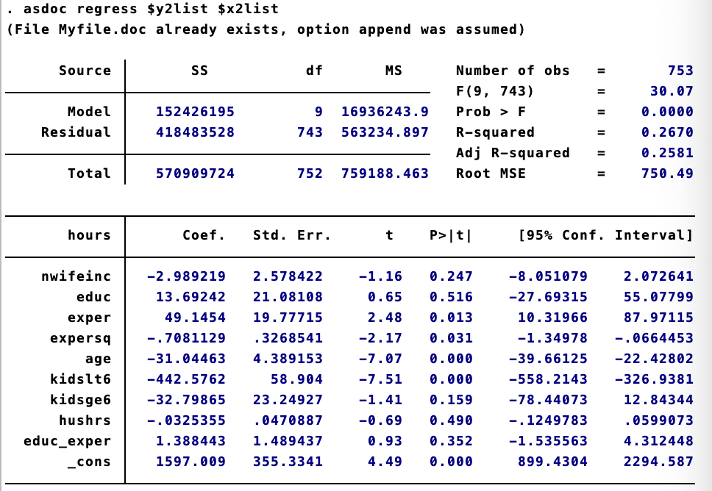
\includegraphics[scale = 0.8]{100_tab_results/MCOensemblepopu.png}
    \centering
    \label{reg:RegressionMCOpopu}
\end{figure}


En estimant le modèle \ref{reg:RegressionMCOpopu} sur l’ensemble de la population, nous sommes dans une situation aussi biaisée. Le problème de générer une telle régression est que nous pouvons faire des prédictions d’heures négatives. Or cette situation n’est pas possible. Nous faisons face à une situation de censure. Nous allons construire un modèle qui permet de borner l’output à 0 (limite basse). Par l’utilisation d’un modèle de censure, un modèle \emph{Tobit}, nous allons atténuer le biais. 
Nous pouvons aussi vérifier la qualité du modèle notamment normalité des résidus. Le test de Jarque-Berra nous indique l’hypothèse nulle de normalité des résidus est rejetée au seuil de 5\%.


\subsubsection{Modèle de sélection Tobit sur l'ensemble de la population.}

Dans cette régression \ref{fig:regTobit}, nous allons censurer le nombre d’heures à 0 (limite inférieur). Néanmoins, en procédant de cette manière, nous sommes aussi confrontés à des problèmes. Nous sommes incapables de différencier les vrais 0. Cela signifie que nous sommes incapables de différencier les individus qui ne souhaitent pas travailler, le salaire de réservation n’est pas suffisamment élevé (salaire minimum à partir duquel l’individu accepte de travailler), des individus qui cherchent en emploi sans succès. Nous estimons le modèle sur l'ensemble de la population : 

\begin{figure}[h]
    \caption{Regression Tobit : modèle censuré, estimation sur l'ensemble de la population.}
    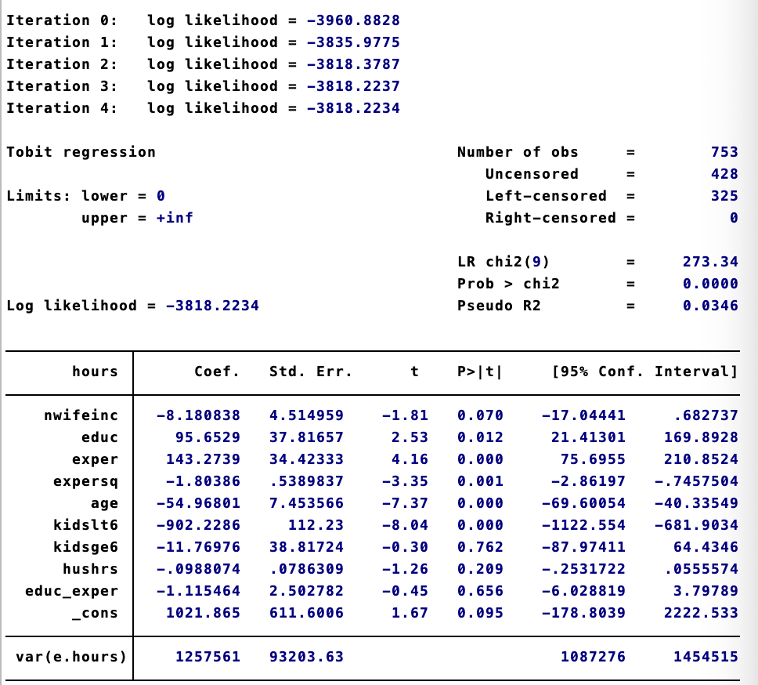
\includegraphics[scale = 0.8]{100_tab_results/tobit.png}
    \centering
    \label{fig:regTobit}
\end{figure}


Aussi, sur un plan économétrique, nous pouvons faire l’analyse des résidus. Le modèle Tobit est construit sur la normalité des résidus. Dans le cadre de ce modèle, nous faisons un test de Jarque-Berra. la normalité des résidus est rejetée au seuil de 5\%, le modèle proposé n’est pas valide. L'histogramme \ref{fig:residuTobit} présente la répartition des résidus.

\begin{figure}[h]
    \caption{Résidu du modèle Tobit.}
    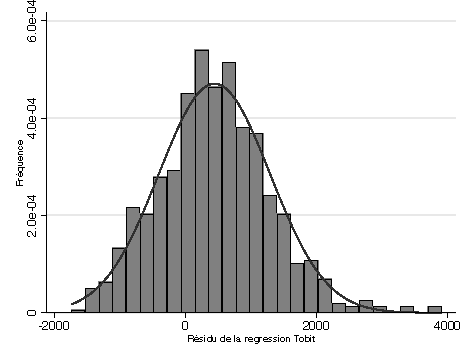
\includegraphics{101_graphics/Tobitresidu.pdf}
    \centering
    \label{fig:residuTobit}
\end{figure}


\vspace*{0.3cm}

Pour faire face à ce problème (différencier les individus), nous pouvons utiliser un modèle de troncature (modèle de \emph{Heckman}). Ce modèle considère que l’échantillon à disposition présente des spécificités et cherche donc à mitiger ce biais de sélection. En effet, dans la construction de cette base, les individus qui travaillent sont sûrement surreprésenté limitant alors l'inférence. L'estimation du modèle de troncature est est donné par la table \ref{reg:HeckmanModel}.

\begin{figure}[!h]
    \caption{Régression d'un modèle de troncature : modèle d'Heckman.}
    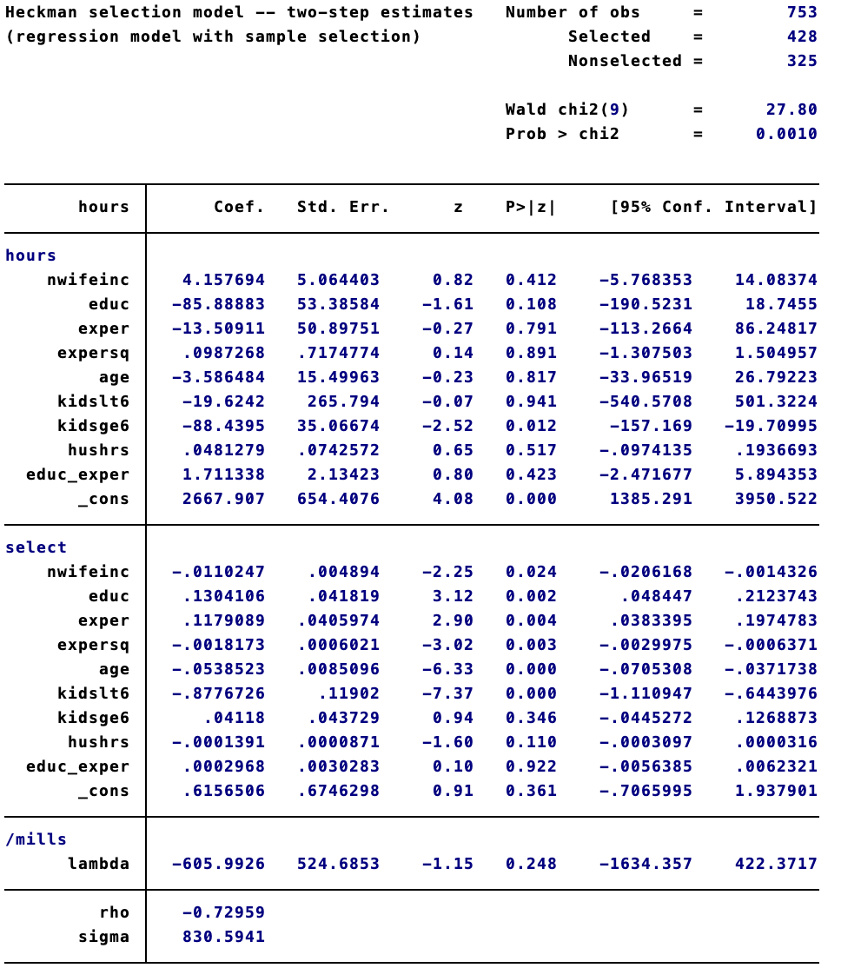
\includegraphics[scale = 0.8]{100_tab_results/Heckman.png}
    \centering
    \label{reg:HeckmanModel}
\end{figure}

\newpage

\subsubsection{Modèles de comptages : Poisson, Binomial négatif, ZIP, ZINP.}


Pour étudier le nombre d'heures travaillées, nous allons présenter des modèles de comptages suivants : 

\begin{itemize}
    \item Modèle de Poisson (\emph{poisson reg}) ;
    \item Modèle Binomial Négatif (\emph{nb reg}) ; 
    \item Modèle Zero Inflated Poisson (\emph{zip reg}) ; 
    \item Modèle Zero Inflated Negative Binomial (\emph{zinb reg}).
\end{itemize}

\subsubsection*{Estimation des modèles.}

Pour faciliter la comparaison entre les modèles, nous présentons ci-dessous un tableau récapitulatif présentant les différents résultats des modèles \ref{tab:countModels} 

\clearpage

\begin{center}
        \small
    {
\def\sym#1{\ifmmode^{#1}\else\(^{#1}\)\fi}
\begin{tabular}{l*{4}{c}}
\hline\hline
            &\multicolumn{1}{c}{(1)}&\multicolumn{1}{c}{(2)}&\multicolumn{1}{c}{(3)}&\multicolumn{1}{c}{(4)}\\
            &\multicolumn{1}{c}{poisson reg}&\multicolumn{1}{c}{nb reg}&\multicolumn{1}{c}{zip reg}&\multicolumn{1}{c}{zinb reg}\\
\hline
hours       &                     &                     &                     &                     \\
nwifeinc    &    -0.00674\sym{***}&     -0.0115         &    0.000171         &   -0.000200         \\
            &    (-46.95)         &     (-1.19)         &      (1.20)         &     (-0.05)         \\
[1em]
educ        &      0.0712\sym{***}&      0.0919         &     -0.0321\sym{***}&     -0.0345         \\
            &     (56.62)         &      (1.27)         &    (-26.17)         &     (-1.20)         \\
[1em]
exper       &       0.135\sym{***}&       0.167\sym{*}  &      0.0277\sym{***}&      0.0280         \\
            &    (128.99)         &      (2.29)         &     (26.39)         &      (1.05)         \\
[1em]
expersq     &    -0.00178\sym{***}&    -0.00234\sym{*}  &   -0.000545\sym{***}&   -0.000595         \\
            &   (-109.94)         &     (-2.05)         &    (-32.80)         &     (-1.43)         \\
[1em]
age         &     -0.0438\sym{***}&     -0.0516\sym{**} &     -0.0154\sym{***}&     -0.0150\sym{*}  \\
            &   (-198.24)         &     (-3.02)         &    (-67.86)         &     (-2.56)         \\
[1em]
kidslt6     &      -0.827\sym{***}&      -1.044\sym{***}&      -0.268\sym{***}&      -0.289\sym{**} \\
            &   (-196.31)         &     (-4.51)         &    (-63.26)         &     (-3.04)         \\
[1em]
kidsge6     &     -0.0362\sym{***}&      0.0430         &     -0.0588\sym{***}&     -0.0588         \\
            &    (-30.82)         &      (0.46)         &    (-48.74)         &     (-1.85)         \\
[1em]
c.educ#c.exper&    -0.00146\sym{***}&    -0.00169         &     0.00107\sym{***}&     0.00119         \\
            &    (-19.90)         &     (-0.32)         &     (15.02)         &      (0.65)         \\
[1em]
\_cons      &       6.816\sym{***}&       6.683\sym{***}&       7.902\sym{***}&       7.914\sym{***}\\
            &    (352.37)         &      (5.47)         &    (414.73)         &     (17.22)         \\
\hline
/           &                     &                     &                     &                     \\
lnalpha     &                     &       2.004\sym{***}&                     &      -0.674\sym{***}\\
            &                     &     (36.80)         &                     &    (-10.57)         \\
\hline
inflate     &                     &                     &                     &                     \\
nwifeinc    &                     &                     &      0.0213\sym{*}  &      0.0213\sym{*}  \\
            &                     &                     &      (2.51)         &      (2.51)         \\
[1em]
educ        &                     &                     &      -0.214\sym{**} &      -0.214\sym{**} \\
            &                     &                     &     (-2.96)         &     (-2.96)         \\
[1em]
exper       &                     &                     &      -0.198\sym{**} &      -0.198\sym{**} \\
            &                     &                     &     (-2.79)         &     (-2.79)         \\
[1em]
expersq     &                     &                     &     0.00315\sym{**} &     0.00315\sym{**} \\
            &                     &                     &      (3.09)         &      (3.09)         \\
[1em]
age         &                     &                     &      0.0881\sym{***}&      0.0881\sym{***}\\
            &                     &                     &      (6.04)         &      (6.04)         \\
[1em]
kidslt6     &                     &                     &       1.443\sym{***}&       1.443\sym{***}\\
            &                     &                     &      (7.09)         &      (7.09)         \\
[1em]
kidsge6     &                     &                     &     -0.0596         &     -0.0596         \\
            &                     &                     &     (-0.80)         &     (-0.80)         \\
[1em]
c.educ#c.exper&                     &                     &   -0.000642         &   -0.000642         \\
            &                     &                     &     (-0.12)         &     (-0.12)         \\
[1em]
\_cons      &                     &                     &      -0.511         &      -0.511         \\
            &                     &                     &     (-0.46)         &     (-0.46)         \\
\hline
\(N\)       &         753         &         753         &         753         &         753         \\
pseudo \(R^{2}\)&       0.263         &       0.006         &                     &                     \\
\textit{AIC}&    630603.4         &      8661.3         &    197595.6         &      7719.8         \\
\textit{BIC}&    630645.0         &      8707.5         &    197678.9         &      7807.6         \\
p           &           0         &    5.92e-09         &           0         &    0.000509         \\
\hline\hline
\multicolumn{5}{l}{\footnotesize \textit{t} statistics in parentheses}\\
\multicolumn{5}{l}{\footnotesize \sym{*} \(p<0.05\), \sym{**} \(p<0.01\), \sym{***} \(p<0.001\)}\\
\end{tabular}
}

    \normalsize
    \label{tab:countModels}
\end{center}


\subsubsection*{Commentaires de la table de résultats.}

\subsubsection*{Le meilleur modèle.}

Tous les modèles sont globalement significatifs (dernière ligne du tableau \emph{p}), il est donc question de trouver quel est le modèle le plus adapté pour modéliser le nombre d'heures travaillées par les femmes en 1975. 

\vspace*{0.3cm}

Le modèle de Poisson indique un $R^2$ plutôt bon pour un modèle non-linéaire (supérieur à 20\%). Néanmoins, nous soulever plusieurs limites de ce modèle : 

\vspace*{0.3cm}

\begin{itemize}
    \item Le modèle est construit sur une hypothèse d'\emph{équidispersion} (c'est-à-dire que si on considère que $y \backsim Poisson(\lambda)$ suit une loi de Poisson alors $E(y)=V(y)=\lambda)$ ; 
    \item Le modèle de Poisson met en valeur beaucoup de 0 (\emph{zero excess burden}).
\end{itemize}

\vspace*{0.3cm}

Pour résoudre ces deux problèmes, nous utilisons le modèle négative binomial qui permet de lever l'hypothèse d'équidispersion, la variance peut être alors différente de la moyenne. Nous pouvons réduire la sureprésentation de zéro à l'aide d'un modèle \emph{zero inflated}. Il apparait que le paramètre \emph{lnalpha} est significatif dans les deux modèles considérant une regression binomiale négative. Cela indique que l'hypothèse nulle du modèle de poisson est rejetée. Nous pouvons donc écarter les modèles de Poisson. 

\vspace*{0.3cm}

En comparant les critères d'information des quatre modèles, le modèle 4 (ZINB) est le meilleur modèle puisqu'il minimise les critères d'information AIC et BIC. Ce modèle (ZINP) malgré un pseudo R2 faible supposé (nous nous appuyons sur le $R^2$ de la modélisation négative binomial), permet de traiter à la fois l'\emph{équidispersion} posé par le modèle de Poisson et la problématique lié à la \emph{surpondérance de zéro} dans la prédiction. 

\subsubsection*{L'interprétation des coefficients.}

Pour la regression de Poisson, le coefficient associé au revenu de transfert de la femme (revenu du conjoint ainsi que les revenus du patrimoine), peut être estimé de la manière suivante : une augmentation d'une unité du revenu de transfert conduit à 0,0061\% d'heures travaillées en moins. Une année d'éducation supplémentaire, conduite à un accroissement du nombre d'heures travaillées de 0,0725\%.

\vspace*{0.3cm}

Si nous interprétons le modèle \emph{Zero Inflated Negativie Binomial}, seules deux variables sont significatives au seuil de 5\% : l'âge de la femme ainsi que le nombre d'enfants ayant moins de 6 ans. L'interprétation est particulière : pour les individus qui travaillent (des heures travaillées supérieures à 0), être agé d'une année supplémentaire conduit à une diminution de 0,015\% d'heures travaillées toute chose égale par ailleurs. Les femmes qui travaillent, qui ont un enfant agé de moins de 6 ans, ont 0,289\% d'heures travaillées en moins. Le reste des coefficients ne sont pas statistiquement significativement différent de 0, et ne donc pas interprétable.